\documentclass[12pt]{book}
\usepackage[utf8]{inputenc}
\usepackage[spanish,es-tabla]{babel}
\decimalpoint
\let\cleardoublepage\clearpage
\usepackage{amsmath}
\usepackage{amsfonts}
\usepackage{amssymb}
\usepackage{color}
\usepackage{graphicx}
\usepackage{makeidx}
\makeindex
\usepackage{anysize}
\usepackage{anyfontsize}
\usepackage{pdfpages}
\usepackage[x11names,table]{xcolor}
\usepackage{tikz}
\usepackage{tcolorbox}
\usepackage[hidelinks]{hyperref}
\usepackage{caption}
\usepackage{listings}
\usepackage{array,ragged2e}
\usepackage[left=2cm,top=2cm,right=2cm,bottom=2cm]{geometry}
\setlength{\parindent}{0cm}
\usepackage[printwatermark]{xwatermark}
\usepackage{xcolor}
\newwatermark[allpages,color=gray!10,angle=45,scale=3,xpos=0,ypos=0]{Borrador}

\tcbset{colback=green!5!white, colframe=gray!10!black, coltitle=green!20!black, 
fonttitle=\bfseries, colbacktitle=white, coltext=gray!30!black}
\addto\captionsspanish{
  \renewcommand{\figurename}{{\bf Figura}}% 
}
\addto\captionsspanish{
  \renewcommand{\chaptername}{{\bf}}% 
}
\usepackage{epigraph}

\newtcolorbox{ejemplo}[2][]
{
  colframe = gray!25,
  colback  = gray!25,
  coltitle = gray!20!black,
  title    = #2,
}

\newtcolorbox{informacion}[2][]
{
  colframe = blue!25,
  colback  = blue!10,
  coltitle = blue!20!black,
  title    = #2,
}

\newtcolorbox{recomendacion}[2][]
{
  colframe = green!25,
  colback  = green!10,
  coltitle = green!20!black,
  title    = #2,
}


% Colores
\definecolor{verdep}{RGB}{166,206,58}
\definecolor{ccap}{RGB}{50,100,50}
\definecolor{csec}{RGB}{50,150,50}
\definecolor{csubsec}{RGB}{50,200,50}
\definecolor{header_table_color}{RGB}{200,255,180}

% Nuevos comandos

\usepackage{titlesec}%--
% \newcommand{\hsp}{\hspace{5pt}}
% \titleformat{\chapter}[hang]{\huge\bfseries\color{ccap}}
% {\color{verdep}{\vrule height 2.5cm width 1mm}\hsp{\fontsize{100}{5}\selectfont\thechapter}\hsp%
% {\vrule height 2.5cm width 1mm}\hsp{\fontsize{30}{5}\selectfont}}{5pt}{\huge\bfseries}

\titleformat{\section}[hang]{\normalfont\color{csec}}%
{\filright\large\enspace\thesection\enspace}%
{8pt}{\Large\bfseries\filright}%

\titleformat{\subsection}[hang]{\normalfont\color{csec}}%
{\filright\large\enspace\thesubsection\enspace}%
{8pt}{\large\bfseries\filright}%

% Code

\lstnewenvironment{matlab}{\lstset{frame=none,
  language=Matlab,
  aboveskip=3mm,
  belowskip=3mm,
  showstringspaces=false,
  columns=flexible,
  basicstyle={\small\ttfamily},
  numbers=none,
  numberstyle=\tiny\color{gray},
  keywordstyle=\color{blue},
  commentstyle=\color{dkgreen},
  stringstyle=\color{mauve},
  breaklines=true,
  breakatwhitespace=true,
  tabsize=3
}}{}

\author{Pedro Jorge De Los Santos}
\title{Programación en MATLAB, fundamentos y aplicaciones}

\begin{document}
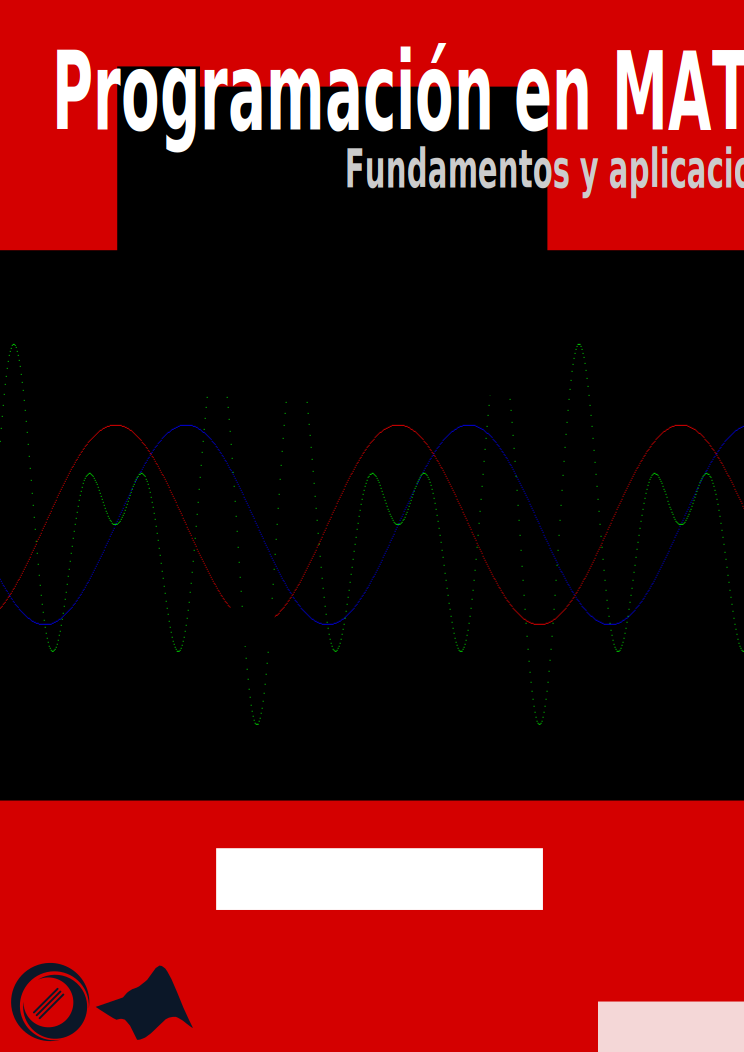
\includepdf{src/portada}
\maketitle
\tableofcontents

\input{src/cfg.tex}

\chapter*{Acerca de...}

\section*{El libro...}

\textbf{Programación en MATLAB, fundamentos y aplicaciones} forma parte del proyecto LAB DLS, cuyo objetivo es
proporcionar herramientas a los usuarios hispanohablantes de MATLAB. %, mediante un blog y un canal de YouTube.\\

El libro consta, por ahora, de 10 capítulos en los cuales se abordan los temas básicos de la programación
en MATLAB y algunas de sus aplicaciones. Los capítulos son:\\

\begin{enumerate}
\item Fundamentos del lenguaje
\item Vectores y matrices
\item Arreglos de celdas, estructuras y cadenas de caracteres
\item Gráficas
\item Exportar e importar variables y datos
\item Matemáticas con MATLAB
\item Procesamiento de imágenes
\item Interfaces gráficas de usuario
\item Programación orientada a objetos
\item Recomendaciones generales
\end{enumerate}

El capítulo 1 abarca los temas introductorios al lenguaje, tales como el uso del entorno de desarrollo, los tipos
de datos y operadores, sentencias de control, ficheros de comandos y funciones.\\

El capítulo 2 proporciona información más detallada acerca de los vectores y matrices, cuya importancia es vital 
para sacar el máximo provecho del lenguaje, dado que es ahí donde reside la popularidad que se ha ganado.\\

El capítulo 3 está destinado a tratar otros tipos de datos más avanzados, pero que de igual forma juegan un
papel muy importante en el aprendizaje. Las cadenas de caracteres se incluyeron en este capítulo con la finalidad
de hacerlas más visibles, dado que muchas veces se tiende a subestimar en este tipo de lenguajes.\\

El capítulo 4 trata un tema muy importante como son las gráficas, en dos y tres dimensiones. Se ofrecen temas
que permiten \textit{estilizar} las gráficas y cómo exportarlas en diversos formatos.\\

El capítulo 5 se ha orientado a las diversas formas de interactuar con datos contenidos en formatos de aplicaciones 
externas, así como el manejo de las variables creadas durante una sesión de MATLAB, y claro, la manipulación de
archivos y directorios utilizando funciones nativas de MATLAB.\\

Los capítulos 6 y 7 muestran algunas aplicaciones de MATLAB en la solución de problemas comunes en matemáticas 
universitarias y procesamiento digital de imágenes, respectivamente.\\

El capítulo 8 es una introducción al desarrollo de interfaces gráficas de usuario en MATLAB, y por tanto se 
abarcan las cuestiones esenciales. Si necesita una mayor referencia en este tema, puede consultar el blog del
proyecto MATLAB TYP, se está trabajando en un texto orientado a este aspecto (Título: Desarrollo de GUIs en MATLAB) 
y se espera que a finales de 2015 esté disponible una versión inicial.\\

El capítulo 9 aborda un tema que generalmente se omite en la mayoría de los libros de esta especie: la programación
orientada a objetos (POO). Se exponen los conceptos básicos de este paradigma de programación, la sintaxis correspondiente 
al lenguaje, la organización de ficheros de clases y el manejo de objetos.\\

El capítulo 10 incluye una serie de recomendaciones que le permitirán al programador en MATLAB el desarrollo de
aplicaciones mejor documentadas, legibles y optimizadas.

\section*{La licencia...}

Este texto se distribuye bajo licencia Creative Commons BY-NC-ND 2.5 MX.\\

En resumen: usted es libre de copiar, compartir y/o distribuir este contenido, siempre y cuando se 
atribuyan los créditos correspondientes al autor del mismo y que no se haga uso de este con fines
comerciales.\\

Para una descripción más detallada de la licencia puede visitar: \url{http://creativecommons.org/licenses/by-nc-nd/2.5/mx/}

% \section*{La tipografía utilizada...}

% \subsection*{Texto}

% El texto ordinario está escrito en fuente tipo [tipo] y tamaño [tam], este parrafo es un ejemplo del mismo.

% \subsection*{Código MATLAB}

% El código MATLAB ha sido resaltado con la finalidad de hacer más legible el texto, por ejemplo:

% \begin{verbatim}	
% 	[x,y]=meshgrid(0:0.1:10);
% 	z = sin(x) + cos(y);
% 	surf(x,y,z);
% 	colormap(hot);
% \end{verbatim}

% \subsection*{Tips de programación}

% Los tips de programación incluyen información que le puede ser útil al usuario al momento de escribir código
% en MATLAB, se distingue del texto ordinario mediante un recuadro como el siguiente:

% \begin{tcolorbox}[title=Tip]
% Bla bla bla bla
% \end{tcolorbox}%


\section*{El autor...}

Ingeniero Mecánico, egresado del Instituto Tecnológico de Tuxtla Gutiérrez en el Sureste de la República
Mexicana y actualmente estudiante de posgrado en el Instituto Tecnológico de Celaya. Programador en 
Python, MATLAB, Java y C/C++.\\

\textit{Pedro Jorge De Los Santos}\\
\textit{delossantosmfq@gmail.com}\\

\href{https://labdls.blogspot.mx}{\includegraphics[scale=0.1]{src/blogger_logo.png}}
\href{https://www.youtube.com/user/lab2dls}{\includegraphics[scale=0.1]{src/youtube_logo.png}}
\href{https://github.com/JorgeDeLosSantos}{\includegraphics[scale=0.08]{src/github_logo.png}}
\href{https://www.linkedin.com/in/pjdlsl}{\includegraphics[scale=0.1]{src/linkedin_logo.png}}
\href{https://plus.google.com/u/0/+pjdelossantos}{\includegraphics[scale=0.1]{src/google_logo.png}}



% Image Download from: https://pixabay.com/en/tiger-animal-relaxation-rest-look-1092497/
\input{src/ch1.tex}
\input{src/ch2.tex}
\chapter{Arreglos de celdas, estructuras y cadenas de caracteres}

\section{Arreglos de celdas}

Un \textit{cell array} \index{cell array} o arreglo de celdas es un arreglo multidimensional que puede 
contener diversos tipos de datos e incluso otro cell array. Suelen utilizarse como agrupadores de datos de diversos tipos.

\subsection{Crear un arreglo de celdas}

La manera más \textit{común} de definir un cell array es utilizando llaves como delimitadores, 
comas y/o puntos y comas como separadores (funcionando de la misma forma que en matrices). 
Por ejemplo:

\begin{verbatim}
	>> A={'Ana',rand(3),true}
	A = 
	    'Ana'    [3x3 double]    [1]
	>> whos
	  Name      Size            Bytes  Class    Attributes
	  A         1x3               415  cell     
\end{verbatim}

Puede notar que se han introducido elementos de diversos tipos y tamaños, aunque claro que funciona 
también para elementos del mismo tipo:

\begin{verbatim}
	>> A={1,2,3;0,2,1;2,3,1}
	A = 
	    [1]    [2]    [3]
	    [0]    [2]    [1]
	    [2]    [3]    [1]
\end{verbatim}

Además, puede definir un arreglo de celdas vacío utilizando la función cell, cuya sintaxis es:

\begin{verbatim}
	>> C = cell(m,n);
\end{verbatim}

Donde m y n especifican el tamaño del arreglo. Una vez creado el cell array vacío puede utilizarse 
la asignación \textit{uno a uno} para rellenar cada posición del mismo, por ejemplo:

\begin{verbatim}
	>> C=cell(2,3);
	>> C{1,1}='A';
	>> C{1,2}='X';
	>> C{1,3}=2;
	>> C{2,1}=true;
	>> C{2,2}=false;
	>> C{2,3}='T';
	>> C
	C = 
	    'A'    'X'    [2]
	    [1]    [0]    'T'
\end{verbatim}

\subsection{Indexado de un cell array}


\section{Estructuras}

Las estructuras (\texttt{struct}) son un tipo de arreglo multidimensional en MATLAB, que permiten almacenar 
datos de diversos tipos, cada dato se almacena en un campo definido mediante un nombre.

\subsection{Crear una estructura de datos}

Una estructura de datos se puede definir utilizando la sintaxis:

\begin{verbatim}
	>> NombreEstructura.NombreCampo = Valor
\end{verbatim}

Donde \textit{NombreEstructura} es el nombre de la estructura, \textit{NombreCampo} el nombre del campo, y \textit{Valor} 
el valor asignado a ese campo de la estructura, el cual puede ser una variable o dato de cualquier tipo, incluyendo 
otros tipos de arreglos o matrices. Note que el nombre de la estructura y el del campo están separados por un punto.\\





\begin{verbatim}
	>> Alumnos.nombre='Juan Pérez';
	>> Alumnos.edad=20;
	>> Alumnos.notas=[10,8,9];
	>> Alumnos
	Alumnos = 
	    nombre: 'Juan Pérez'
	      edad: 20
	     notas: [10 8 9]
	>> whos Alumnos
	  Name         Size            Bytes  Class     Attributes

	  Alumnos      1x1               580  struct      
\end{verbatim}

\subsection{Accediendo a campos de una estructura}



\section{Cadenas de caracteres}

Las cadenas de caracteres o strings (aquí usaremos indistintamente ambos términos) son un tipo 
de dato común en la mayoría de los lenguajes de programación de alto nivel, consisten en una 
serie de caracteres que representan una palabra, frase, texto o cualquier otra representación 
mediante símbolos propios de un sistema de escritura.\\

Como ya sabemos en MATLAB no hace falta declarar el tipo de cada variable, pero es necesario 
utilizar cierta sintaxis para que el intérprete reconozca cada tipo de dato, así, para crear 
una cadena de caracteres es necesario delimitar su contenido entre comillas simples, por ejemplo:

\begin{verbatim}
	>> txt='Programación en MATLAB'
	txt =
	Programación en MATLAB
	>> whos
	  Name      Size            Bytes  Class    Attributes
	  txt       1x22               44  char    
\end{verbatim}

\subsection{Concatenación}

La concatenación de cadenas de caracteres es la operación de unir dos o más cadenas en una nueva. 
Una forma de concatenar strings es utilizando la notación de corchetes, véase el ejemplo a continuación:

\begin{verbatim}
	>> cad1='Hola, ';
	>> cad2='bienvenido';
	>> cad3=' a este curso de MATLAB';
	>> cad_res=[cad1,cad2,cad3]
	cad_res =
	Hola, bienvenido a este curso de MATLAB
\end{verbatim}

Además de lo anterior MATLAB también dispone de una función \textit{especializada}  para esta tarea: 
strcat. La sintaxis es muy sencilla, a saber:

\begin{verbatim}
	>> concStr=strcat(s1, s2, s3, …, sN);
\end{verbatim}

Siendo concStr la cadena resultante, y s1, s2, s3 y sN una lista de strings separadas por comas, 
y que son los que habrán de concatenarse. Por ejemplo:

\begin{verbatim}
	>> cad=strcat('Esto es una',' cadena concatenada',' con strcat')
	cad =
	Esto es una cadena concatenada con strcat
\end{verbatim}


\begin{tcolorbox}[title=De la concatenación]
En muchos otros lenguajes de programación es común utilizar el operador de suma (+) para la concatenación de strings, 
por lo cual puede resultar \textit{tentador} intentarlo en MATLAB, pero  esto produce un resultado diferente al esperado. 
Lo que MATLAB hace es sumar elemento a elemento el valor correspondiente en código ASCII de cada una de las letras 
que componen el arreglo de caracteres, por lo cual se deduce además que es imposible operar de esta forma con cadenas 
de longitudes diferentes. Luego, si se suman dos cadenas de igual longitud, entonces MATLAB devolverá un vector de 
tipo double.
\end{tcolorbox}


\subsection{Mayúsculas y minúsculas}

Si necesita representar una cadena de caracteres solo mediante mayúsculas o minúsculas, MATLAB 
proporciona funciones para cada caso. Con upper se convierte una cadena pasada como argumento 
en su representación en mayúsculas:

\begin{verbatim}
	>> s=upper('hola mundo')
	s =
	HOLA MUNDO
\end{verbatim}

Usando lower puede hacerlo para el caso de minúsculas:

\begin{verbatim}
	>> s=lower('MATLAB es divertido')
	s =
	matlab es divertido
\end{verbatim}

\subsection{Buscar y remplazar strings}

\subsubsection{Buscar en una cadena de texto}

Actualmente es común que millones de personas busquen a diario en el internet cualquier 
diversidad de temas o palabras claves de algún interés, obteniendo respuesta en milésimas 
de segundo. Claro que los algoritmos de búsqueda que implementan los buscadores de la web 
como el omnipresente Google son muy sofisticados y basan sus resultados en conceptos muy 
definidos de clasificación y relevancia.\\

En esta sección veremos como MATLAB permite \textit{buscar} palabras, frases y caracteres 
dentro de una cadena de texto. Obviando las diferencias de complejidad y utilidad, esto es 
muy similar a lo mencionado en líneas anteriores.\\

La función más común para buscar un determinado patrón de caracteres es strfind cuya sintaxis es:

\begin{verbatim}
	>> strfind(texto, busca);
\end{verbatim}

Donde texto es la cadena de caracteres en donde se buscará el patrón definido en la 
variable busca. Y  como es \textit{costumbre} en este texto, iremos a por un ejemplo:

\begin{verbatim}
	>> texto='Anita lava la tina';
	>> busca='lava';
	>> strfind(texto,busca)
	ans =
	     7
\end{verbatim}

Y ahora, ¿por qué nos devuelve un 7?, MATLAB devuelve la posición en la cual inicia el patrón 
o cadena buscada, en este caso la palabra lava comienza en la posición 7 de texto. Un ejemplo más:

\begin{verbatim}
	>> texto='Este es otro ejemplo';
	>> busca='o';
	>> strfind(texto,busca)
	ans =
	     9    12    20
\end{verbatim}

Puede notar que en este caso MATLAB devuelve más de un resultado, lo cual indica claramente 
que el carácter buscado se encuentra más de una vez dentro del texto, y al igual que lo 
anterior estos números indican la posición inicial del carácter o cadena buscada.\\

Puede ser que la utilidad de la función strfind hasta este punto le parezca cuasi nula, démosle 
entonces una aplicación más \textit{tangible}: dada una cadena de texto y un patrón de búsqueda, 
eliminaremos cada coincidencia encontrada:

\begin{verbatim}
	>> texto='Eliminando la vocal i de esta frase';
	>> busca='i';
	>> k=strfind(texto,busca);
	>> texto(k)='' % Eliminamos coincidencias
	texto =
	Elmnando la vocal  de esta frase
\end{verbatim}

Es posible que haya notado que incluso puede remplazar cada coincidencia por otra letra y no 
necesariamente por un string vacío. Lo anterior funciona solamente para patrones de búsqueda 
cuya longitud sea unitaria, para el resto de casos debe sustituir la última línea por:

\begin{verbatim}
	>> texto(k:k+length(busca))=''
\end{verbatim}

\subsubsection{Remplazando en una cadena de texto}

Hemos visto como buscar y luego reemplazar cierto patrón buscado en una cadena de caracteres, 
mediante la indexación de cada coincidencia, pero MATLAB \textit{facilita} el trabajo y 
proporciona la función \texttt{strrep} que reemplaza las coincidencias encontradas, la sintaxis es:

\begin{verbatim}
	>> modStr=strrep(origStr,  anterior, nuevo)
\end{verbatim}

Donde origStr es la cadena de caracteres original, anterior es el valor o parte de la cadena a 
remplazar, nuevo es el valor por el cual será remplazado, y modStr la cadena resultante al 
remplazar los valores especificados. Enseguida se muestra un ejemplo, utilizando el clásico 
trabalenguas de los tigres y trigos:

\begin{verbatim}
	>> s='tres tristes tigres tragaban trigo';
	>> srep=strrep(s,'tr','tl')
	srep =
	tles tlistes tigres tlagaban tligo
\end{verbatim}

Tal como se observa, se ha remplazado toda aparición conjunta de las letras tr por tl, conllevando 
ello a una versión \textit{enrarecida} de tan magnífico ejercicio de expresión oral.\\

La función \texttt{strrep}, como se ha visto, proporciona una herramienta para reemplazar ciertos 
valores en una cadena de caracteres, pero también está limitada a que los valores pasados como 
argumentos de entrada deben ser exactos, sin permitir flexibilidad alguna al momento de definir 
los patrones de búsqueda. Desde luego que lo anterior tiene una solución práctica y muy conocida 
en el mundo de la programación: las expresiones regulares, que se estarán tratando en una sección posterior.

\subsection{Comparar cadenas de caracteres}

Comparar cadenas de caracteres resulta muy útil en casos que se necesite hacer una selección o 
toma de decisión dependiendo de una variable cuyo valor sea un string. Para tal fin se utiliza 
la función \texttt{strcmp} devuelve un valor lógico verdadero si las cadenas comparadas son iguales 
y falso en caso contrario, la sintaxis es:

\begin{verbatim}
	>> strcmp(str1, str2);
\end{verbatim}

Donde str1 y str2 son las cadenas a comparar. Revise los siguientes ejemplos:

\begin{verbatim}
	>> strcmp('MATLAB','MATLAB')
	ans =
	     1
	>> strcmp('MATLAB','matlab')
	ans =
	     0
\end{verbatim}

Del último ejemplo puede deducir que la función strcmp es case-sensitive y aun cuando las cadenas 
sean iguales y difieran únicamente por el uso de mayúsculas o minúsculas, MATLAB devolverá un 
valor false. Para ignorar o evitar que se tome en cuenta el uso de mayúsculas o minúsculas puede 
emplear previamente una conversión a cualquiera de los casos, por ejemplo:

\begin{verbatim}
	>> strcmp(lower('MATLAB'),lower('matlab'))
	ans =
	     1
\end{verbatim}

Por alguna razón la solución anterior podría parecerle poco elegante, quizá lo mismo pensaron 
los desarrolladores de MathWorks y decidieron ofrecer una función muy similar a strcmp, con 
la diferencia de ser case-insensitive, hablamos de strcmpi: 

\begin{verbatim}
	>> strcmpi('MATLAB','matlab')
	ans =
	     1
\end{verbatim}

\subsection{Expresiones regulares}
\input{src/ch4.tex}
\chapter{Exportar e importar variables y datos}

\section{Guardar y cargar variables del workspace: save y load}

Durante una sesión ordinaria utilizando MATLAB las variables creadas se almacenan en el 
workspace y están disponibles para usarse, siempre y cuando no se haya utilizado algún 
comando para borrar las variables, sin embargo cuando se cierra la sesión de MATLAB las 
variables del workspace son borradas y no es posible utilizarlas posteriormente. Para 
poder “conservar” una variable creada y utilizarla en cálculos futuros, es posible 
guardar estas en archivos MAT nativos del lenguaje MATLAB; lo anterior se logra utilizando 
la función save, cuya sintaxis es:

\begin{verbatim}
	save('nomb_arch.mat','nvar');
\end{verbatim}

Siendo \texttt{nomb\_arch} el nombre del archivo en el cual se guardarán las variables, 
que incluso puede ser una combinación de una dirección absoluta o relativa y el nombre 
del archivo; nvar es el nombre de la variable o variables a ser guardadas. Si desea 
guardar todas las variables actuales puede omitir el resto de argumentos y solo 
utilizar el nombre del archivo. Las siguientes líneas ejemplifican cómo hacer uso 
de la función save:

\begin{verbatim}
	>> k=1.37;
	>> A=[1 2 -1;0 1 0;-2 0 0];
	>> C={'A','B','C'};
	>> save('arch1.mat'); % Guarda todas las variables
	>> save('arch2.mat','A'); % Guarda sólo la variable A
\end{verbatim}

El contenido de los archivos MAT puede cargarse y guardar en el workspace mediante 
la función \texttt{load}, con la sintaxis:

\begin{verbatim}
	load('narch.mat','vars');
\end{verbatim}

Donde narch es el nombre del archivo y vars la(s) variable(s) a cargar en el workspace. 
Si únicamente se indica como argumento el nombre del archivo, entonces se cargan todas 
las variables contenidas en el archivo. Para ejemplificar el uso de load utilizaremos 
el archivo “arch1.mat” creado anteriormente:

\begin{verbatim}
	>> load('arch1.mat');
	>> whos % Verificamos las variables cargadas en el workspace
	  Name      Size            Bytes  Class     Attributes
	  A         3x3                72  double              
	  C         1x3               342  cell                
	  k         1x1                 8  double       
\end{verbatim}

Puede asignarse la función load a una variable, con lo cual todo el contenido del 
archivo MAT se guardara en una estructura con cada una de las variables como campos. 
Para el mismo ejemplo anterior se tiene:

\begin{verbatim}
	>> S=load('arch1.mat');
	>> S
	S = 
	    k: 1.3700
	    A: [3x3 double]
	    C: {'A'  'B'  'C'}
	>> whos 
	  Name      Size            Bytes  Class     Attributes
	  S         1x1               950  struct       
\end{verbatim}


\section{Carpetas y archivos, operaciones básicas.}

\subsection{Cambiar el directorio o carpeta actual}

La función cd cambia la carpeta actual (Current Folder), utilizando como argumento 
una cadena de caracteres con la dirección absoluta o relativa del nuevo directorio 
de trabajo. La sintaxis es:

\begin{verbatim}
	cd('Nueva Carpeta');
\end{verbatim}

Un ejemplo se muestra enseguida:

\begin{verbatim}
	cd('C:\Users\User\Documents\MATLAB');
\end{verbatim}

Si solo se pone la instrucción \texttt{cd} sin argumentos, entonces MATLAB devuelve un 
string con la carpeta actual.

\begin{quote}
\textbf{Direcciones absolutas y relativas}.\\
Una dirección absoluta es aquella representada mediante toda la ruta que la describe, 
incluyendo al directorio raíz. En Windows las direcciones absolutas suelen ser de la forma 
\texttt{C:/Users/User/…}, donde User es el nombre del usuario registrado en el equipo.
Las direcciones relativas se expresan con respecto a una determinada carpeta, por ejemplo, 
si estamos ubicados dentro de una carpeta Documents cuya dirección absoluta es 
\texttt{C:/Users/User/Documents} y dentro de ella tenemos una carpeta llamada MATLAB, la forma 
relativa de referirnos a esta carpeta sería simplemente con la cadena \texttt{'\MATLAB'}.
\end{quote}

\subsection{Crear y eliminar carpetas}

A estas alturas, crear y manipular carpetas resulta una tarea trivial cuando se ejecuta 
en el ambiente de cualquier sistema operativo que maneje, incluso en el Current Folder 
de MATLAB puede crear, modificar y eliminar carpetas tal como lo hace normalmente. Pese 
a lo anterior, en diversas situaciones puede ser necesario crear carpetas mediante la 
ejecución de código a través de comandos y/o funciones destinadas para tal fin. En MATLAB 
se dispone de la función mkdir que permite crear carpetas utilizando el nombre de la 
misma como argumento, por ejemplo:

\begin{verbatim}
	>> mkdir('Mis Cursos');
\end{verbatim}

La instrucción anterior crea una carpeta llamada Mis Cursos en el directorio actual de 
trabajo. Es posible también pasar como argumento la dirección absoluta o relativa de 
la carpeta a crear:

\begin{verbatim}
	>> mkdir('Mis Cursos/MATLAB');
\end{verbatim}

En la línea anterior se crea dentro de la carpeta Mis Cursos una cuyo nombre es MATLAB.

Habitualmente en la programación se hace necesario considerar la mayoría de las 
situaciones posibles para dar una mayor robustez al código, y con ello hacerlo más 
autónomo y eficiente. Imagine que necesite crear carpeta a la cual le asignará un 
nombre determinado, entonces, hay una posibilidad, aun siendo mínima, que ya exista 
una carpeta con ese mismo nombre. MATLAB no remplazará la carpeta existente por la nueva, 
pero le mostrará un mensaje de error o advertencia y posiblemente detenga la ejecución 
del código. Para evitar lo anterior puede comprobar antes si existe un directorio con 
ese nombre y mediante una sentencia de control especificar las acciones a ejecutar en 
cada caso. Véase el ejemplo siguiente en donde se realiza la comprobación mediante 
la función isdir:

\begin{verbatim}
	if ~isdir('Cursos')
	    mkdir('Cursos');
	else
	    mkdir(['Cursos','2']);
	end
\end{verbatim}

Para eliminar una carpeta MATLAB proporciona la función rmdir cuyo argumento es la 
carpeta a eliminar, o bien la dirección absoluta o relativa de la misma. Por ejemplo, 
si quiere eliminar una carpeta llamada Cursos, ubicada en el directorio actual:

\begin{verbatim}
	>> rmdir('Mis Cursos');
\end{verbatim}

Lo anterior funciona para carpetas que no contengan subcarpetas, de lo contrario 
MATLAB le devolverá un mensaje de error como el siguiente:

\begin{verbatim}
	>> rmdir('Mis Cursos')
	Error using rmdir
	No directories were removed.
\end{verbatim}

Para borrar una carpeta que contenga subcarpetas debe incluir un segundo argumento, 
siendo este una “s” entre comillas simples, como se muestra:

\begin{verbatim}
	>> rmdir('Mis Cursos','s');
\end{verbatim}

\subsection{Crear y eliminar carpetas}

Conocer los archivos y directorios dentro de una carpeta suele ser una necesidad 
básica para cualquier programador, sobre todo para el almacenamiento y organización 
de archivos de trabajo. MATLAB cuenta con funciones que facilitan la tarea de consultar 
el contenido de una carpeta, entre las más comunes están dir, ls y what, a continuación 
veremos la utilidad de cada una.

\subsubsection{La función dir}

La función dir, sin argumentos de salida pedidos de forma explícita y sin argumentos 
de entrada, devuelve en pantalla una lista de archivos y directorios contenidos en 
el \textbf{Current Folder}. Véase el ejemplo:

\begin{verbatim}
	>> dir
	.               grlev.png       matricesEx.m    
	..              idmat.m         ordseleccion.m  
	datos.txt       img.png         unos.m     
\end{verbatim}

No obstante, si asignamos la función dir a una variable cualesquiera entonces se 
guardará una estructura que contiene información acerca del nombre, tamaño, fecha 
de modificación, entre otras características de los archivos contenidos en el 
directorio actual.

\begin{verbatim}
	>> S=dir
	S = 
	9x1 struct array with fields:
	    name
	    date
	    bytes
	    isdir
	    datenum
\end{verbatim}

Para acceder a la información de cada archivo puede hacerlo mediante el índice 
correspondiente, por ejemplo:

\begin{verbatim}
	>> S(3)
	ans = 
	       name: 'datos.txt'
	       date: '01-oct-2014 15:13:46'
	      bytes: 74
	      isdir: 0
	    datenum: 7.3587e+05
\end{verbatim}

Desde luego que esta forma de utilizar la función dir es mucho más útil que aquella 
que simplemente muestra en pantalla la información.

Es posible además especificar como argumento la dirección de la cual se requiere 
información (una distinta al Current Folder) e inclusive utilizar comodines para 
visualizar solo archivos con una determinada extensión, por ejemplo:

\begin{verbatim}
   	>> dir('C:/Users/User/Documents/MATLAB/*.png')
	ayuda.png  img.png 
\end{verbatim}   

La instrucción anterior busca en la carpeta MATLAB todos los archivos con 
extensión PNG (imágenes), sin importar el nombre de estos, e ignora cualquier 
otro tipo de archivo o directorio ubicado en esta misma carpeta. Ahora, 
revise el siguiente ejemplo:

\begin{verbatim}
	>> dir('C:/Users/User/Documents/MATLAB/m*')
	MATLAB TYP           Mecanismos           My File Exchange     
	MATLAB_Function.m    Mis Apuntes          matrizBinaria.m      
	Matemáticas Básicas  Moler Books          miHist.m       
\end{verbatim}

Como puede observar, MATLAB devuelve todos aquellos archivos y carpetas cuya 
primera letra sea \textbf{m}, sin importar ninguna otra característica.

\subsection{Mover, copiar y eliminar archivos}

Mover, copiar y eliminar archivos son tareas muy comunes para cualquier usuario  
de un ordenador y que pueden ejecutarse con mucha facilidad de forma manual. No 
obstante, utilizar la programación para estas tareas puede resultar de mucha ayuda, 
sobre todo cuando se necesita trabajar con grandes volúmenes de datos y/o archivos, 
ya que permite automatizar los procedimientos y ejecutarlos en un tiempo impensable 
para un individuo. Claro que se podría justificar que existen formas para seleccionar 
todos los archivos de un directorio y colocarlos en otro de forma muy sencilla  aun 
cuando fuesen millares de archivos, pero ¿qué pasa si solo necesitamos trabajar con 
archivos cuyo nombre cumpla una determinada característica o patrón? ¿O con archivos 
de un tamaño específico? ¿O con una fecha de modificación reciente?, incluso con 
combinaciones de las anteriores posibilidades, de esa manera no es tan trivial 
seleccionar de forma manual archivos que cumplan tales condiciones, pero utilizando 
la programación puede solucionar de forma efectiva dichas situaciones.

MATLAB proporciona funciones que sirven para realizar las tareas mencionadas en el 
párrafo anterior. Con movefile y copyfile puede mover y copiar archivos de un directorio 
a otro, la sintaxis es muy similar, necesitando solamente el directorio origen y destino 
como argumentos de entrada. Usaremos movefile para ejemplificar, pero desde luego que esto 
será aplicable para copyfile con tan solo cambiar el nombre de la función.

\section{Exportar e importar datos de un fichero de texto}

Existen múltiples formatos para ficheros que almacenan datos o texto plano, siendo los 
más comunes el *.txt y el *.dat. Estos tipos de ficheros son muy utilizados en casi 
cualquier ámbito para guardar datos de cualquier tipo, con la ventaja de ser \textit{leíbles}
para una persona y, por supuesto, para la computadora. Por tanto, con frecuencia se hace 
necesario el hecho de importar y/o exportar información de un archivo de este tipo, además 
es muy común utilizar MATLAB como un entorno de visualización de datos generados a través 
de la adquisición mediante tarjetas o bien mediante otro software.

\subsection{Exportar datos con dlmwrite}

La función dlmwrite exporta el contenido de una matriz a un archivo de texto usando 
un delimitador o separador entre los elementos. La sintaxis más común es:

\begin{verbatim}
	>> dlmwrite(n_arch, M, 'delimitador');
\end{verbatim}

Donde \texttt{n\_arch} es el nombre del archivo en el cual se guardará la matriz M, utilizando 
como separador el carácter especificado en \texttt{'delimitador'}.
\input{src/ch6.tex}
\chapter{Procesamiento de imágenes}

El procesamiento digital de imágenes (PDI o DIP por sus siglas en inglés) es un campo de 
investigación científica muy interesante y cuyas aplicaciones son tan diversas, tales 
como la medicina, el control de calidad en la industria, astronomía, visión artificial, etc. 
Lo anterior nos hace deducir que para abarcar "decentemente" la mayoría de los tópicos 
comunes del PDI se necesitaría más de un libro completo, por lo cual se pretende aclarar 
que en este capítulo se tratarán solamente algunos temas con un nivel de detalle elemental, 
con la esperanza de que sirva al amable lector como una breve introducción y sobre todo, 
en medida de lo posible, motivarle para adentrarse en tan maravilloso mundo.

\section{Conceptos iniciales del procesamiento de imágenes}

\subsection{¿Qué es el procesamiento de imágenes?}

El procesamiento digital de imágenes  es el conjunto de técnicas aplicadas a imágenes 
digitales con un cierto objetivo, los cuales pueden ser: mejorar la calidad de la imagen, 
detección/reconocimiento de formas o colores, realce de ciertas regiones de la imagen, etc.

\subsection{Aplicaciones del procesamiento de imágenes}
 
\section{Importar y mostrar imágenes}

En MATLAB, como en cualquier otro software de procesamiento, las imágenes son tratadas 
como matrices, cuyos elementos corresponden a un valor especifico de cada píxel que la 
compone. La función \texttt{imread} permite leer/importar imágenes en casi cualquier formato 
conocido (*.bmp, *.png, *.tiff, *.jpg, etc). La sintaxis de \texttt{imread} es muy simple, basta 
con pasar como argumento la dirección absoluta o relativa del archivo correspondiente a 
la imagen de interés, por ejemplo la siguiente instrucción lee la imagen “img.jpg” ubicada 
en la carpeta de trabajo (Current Folder).

\begin{verbatim}
	>> A=imread('img.png');
\end{verbatim}

Con el comando \texttt{whos} podemos verificar el tipo de dato con el cual MATLAB guarda la imagen importada:

\begin{verbatim}
	>> whos
	  Name        Size                Bytes  Class    Attributes
	  A         300x400x3            360000  uint8    
\end{verbatim}

MATLAB guarda la información del color de cada píxel que compone la imagen utilizando 
una matriz de tres dimensiones; las dos primeras determinan el tamaño de la imagen y la 
tercera corresponde a cada una de las capas RGB, es decir, en una matriz de mxn elementos 
se guarda la información correspondiente al color rojo, en otras similares las de color 
verde y azul. Por defecto el tipo de dato utilizado para la manipulación de imágenes 
es el uint8 (sin signo de 8 bits).\\

Para mostrar una imagen que ha sido previamente leída con imread se puede utilizar la 
función \texttt{imshow}. Véase el siguiente ejemplo:

\begin{verbatim}
	>> A=imread('imag.jpg');
	>> imshow(A);
\end{verbatim}

\begin{center}
\includegraphics[scale=0.7]{src/ch7/holland_imshow.png}
\captionof{figure}{Bla bla}
\end{center}

La función \texttt{imshow} abre una nueva ventana (figure) y muestra la imagen que ha sido 
guardada con anterioridad  (ver figura 7.1). MATLAB dispone de otras funciones como 
\texttt{image} e \texttt{imagesc}  que también muestran en pantalla las imágenes, pero que suelen 
utilizarse más para la visualización en análisis de datos.

\section{Operaciones básicas con imágenes}

\subsection{Operaciones aritméticas}

Recuerde que una imagen en MATLAB se almacena como una matriz de mxnxp dimensiones, 
luego, es posible realizar operaciones aritméticas de suma, resta y multiplicación sobre 
ella como una matriz común, tal como se ha visto en Capítulo 2.

\subsubsection{Suma de un escalar}

Si sumamos una constante k a una matriz \textbf{A}, entonces cada elemento de \textbf{A} se incrementa en k 
unidades, lo cual se traduciría en un aumento del brillo en la imagen. Véase el ejemplo siguiente:

\begin{verbatim}
	A=imread('imag.jpg');
	k=50;
	A=A+k;
	imshow(A);
\end{verbatim}

\begin{center}
\includegraphics[scale=0.7]{src/ch7/holland_original.png}
\captionof{figure}{Imagen original}
\end{center}

\begin{center}
\includegraphics[scale=0.7]{src/ch7/holland_mas50.png}
\captionof{figure}{Imagen aumentada en 50 unidades}
\end{center}

La imagen 7.2 corresponde a la original y en la 7.3 se muestra lo que resulta de aumentar 
en 50 unidades cada uno de los pixeles que componen la imagen.

\subsubsection{Resta de un escalar}

Es evidente que la resta de un escalar es muy similar en interpretación a la suma vista 
anteriormente, solo que en este caso cada elemento de la matriz disminuye en un valor 
constante. Véase el ejemplo:

\begin{verbatim}
	A=imread('img.jpg');
	k=80;
	A=A-k;
	imshow(A);
\end{verbatim}

\begin{center}
\includegraphics[scale=0.7]{src/ch7/holland_menos50.png}
\captionof{figure}{Imagen disminuida en 50 unidades}
\end{center}

\subsection{Conversión a escala de grises}

La escala de grises es una forma de representar imágenes digitales utilizando solamente variaciones 
de grises, desde negro a blanco.\\

En MATLAB se dispone de la función \texttt{rgb2gray} para convertir una imagen dada en el modelo de color RGB 
a una imagen en escala de grises.

\begin{verbatim}
X=imread('img.png');
XG=rgb2gray(X);
imshow(XG);
\end{verbatim}

\begin{center}
\includegraphics[scale=0.7]{src/ch7/holland_gris.png}
\captionof{figure}{Imagen en escala de grises}
\end{center}

\subsection{Binarización de una imagen}

\section{Segmentación de imágenes}

\subsection{Umbralización}

\subsection{Detección de bordes}

\section{Restauración y mejoramiento de imágenes}

\subsection{Removiendo ruido}
\chapter{Introducción a las GUIs MATLAB}

Una interfaz gráfica de usuario (GUI) es un elemento gráfico que contiene uno o más controles que están disponibles 
para interactuar con el usuario mediante un entorno visual sencillo, el cual permite la comunicación entre el usuario 
y el computador. Entre algunos de los componentes más comunes de una GUI creada en MATLAB se tienen menús, barras de 
herramientas, botones, menús desplegables, cajas de texto, entre otros.\\

En las interfaces gráficas creadas en MATLAB pueden aprovecharse todas las herramientas matemáticas y de ingeniería 
que proporciona MATLAB, permiten además la manipulación de archivos de datos, así como la interacción con otras GUIs 
y mostrar datos mediante tablas y gráficas de gran calidad.\\

Generalmente las GUIs son programadas para que respondan a la manipulación del usuario con una acción específica. 
Los controles gráficos que componen una GUI están relacionados con una rutina de programación, llamada callbacks 
en el entorno MATLAB, que se ejecuta cuando sucede  un determinado evento, que puede ser la entrada de caracteres 
mediante el teclado, el clic de un botón del mouse, o situarse sobre un objeto.

\section{Elemento figure}

En MATLAB cada interfaz gráfica está creada sobre un objeto figure, en este elemento se añaden 
todos los controles gráficos que componen la GUI. La forma más simple de definir un objeto 
figure se ejemplifica enseguida:

\begin{verbatim}
	hFig = figure;
\end{verbatim}

Donde \texttt{hFig} es el handle del elemento figure.\\

Es muy común que al momento de definir o crear un objeto figure, se especifiquen algunas 
de sus propiedades con la sintaxis siguiente:

\begin{verbatim}
	hFig = figure('Propiedad ', 'Valor ',...);
\end{verbatim}

A continuación se muestra un ejemplo característico:

\begin{verbatim}
	hFig = figure('NumberTitle','off',...
	              'MenuBar','None',...
	              'Name','Figure Ejemplo',...
	              'Position',[200 200 300 300]);
\end{verbatim}

Las propiedades más comunes de un elemento figure se muestran en la tabla siguiente:

\begin{table}[h!]
\centering
{\rowcolors{1}{}{gray!20}
\begin{tabular}{p{3cm} p{12cm}}
\rowcolor{LightBlue2} \textbf{Propiedad} & \textbf{Descripción} \\
\texttt{Color} & Establece el color de figure. El valor puede establecerse mediante 
un vector de tres elementos en formato RGB \\

\texttt{MenuBar} & Oculta o muestra la barra de menús estándar de MATLAB \\

\texttt{Name} & Título mostrado en la ventana de la figura. El valor especificado es una cadena de caracteres \\

\texttt{NumberTitle} & Determina si la numeración de los elementos figure creada automáticamente por MATLAB será visible. El valor por defecto es on, para ocultar deberá especificarse off. \\

\texttt{Position} & Especifica el tamaño de la GUI y la posición relativa a la esquina inferior
izquierda de la pantalla. El valor se establece mediante un vector de cuatro
elementos cuya estructura es la siguiente: [Distancia de la
izquierda, Distancia de la parte inferior, Ancho, Alto]; \\

\texttt{Resize} & Determina si puede modificarse el tamaño de la GUI utilizando el mouse. Los
valores aceptados son: off y on, siendo este último el valor por defecto. \\

\texttt{Toolbar} & Muestra o borra el menú de herramientas del objeto figure. \\

\texttt{Units} & Unidad de medida que se utilizará para interpretar el vector de la propiedad
position. Los valores disponibles son: centimeters, characters,
inches, normalized, point y pixels. Siendo este último el valor por defecto. \\

\texttt{Visible} & Establece si la GUI es visible. Valores: on y off. \\

\end{tabular}
\caption{Propiedades de \texttt{figure}}
\end{table}



\section{Controles gráficos (uicontrol)}

Los controles gráficos son creados mediante la función uicontrol, cuya estructura general se muestra:

\begin{verbatim}
	hCont = uicontrol('Style', 'tipo de control',...
	                  'Propiedad', 'Valor');
\end{verbatim}

La propiedad \texttt{style} define el tipo de control gráfico
\input{src/ch9.tex}
\input{src/ch10.tex}

\printindex

\end{document}